\chapter{Literature Review}
\label{ch:lit}
\section{Introduction}

This chapter moves from general image processing to ECG-specific methods, classifiers and existing systems, and argues that image-based ECG classifiers have mostly been tested on synthesised images, with little attention to their confidence and explanations. Abbreviations and technical terms are defined in the Glossary.

\section{Digital Image Processing}
\label{sec:image-processing}

A digital image is a two-dimensional function $f(x,y)$ whose value at each pixel is the intensity at that point \cite{gonzalez_digital_2018}. The intensity is the product of the illumination $i$ and the reflectance $r$ of the surface, $f(x,y) = i(x,y)\,r(x,y)$ \cite{stockham_image_1972}, so one object, or one ECG trace, can look different under different lighting. Images are digitised by sampling into pixels and quantising each value to a finite number of levels, which discards detail irreversibly \cite{gonzalez_digital_2018}.

Processing then enhances the image for a task, removes noise, and segments it into meaningful regions. Table~\ref{tab:techniques} summarises the main techniques and their trade-offs. No single method suits every image, as removing noise can also distort real detail, so the choice depends on the degradation and the task \cite{qi_comprehensive_2022}.

\begin{table}[!htbp]
  \centering
  \footnotesize
  \renewcommand{\arraystretch}{1.15}
  \caption{Image processing techniques relevant to ECG images, and their trade-offs.}
  \label{tab:techniques}
  \begin{tabular}{@{}p{0.27\linewidth} p{0.30\linewidth} p{0.37\linewidth}@{}}
    \toprule
    \textbf{Technique} & \textbf{Use} & \textbf{Trade-off} \\
    \midrule
    Histogram equalisation (HE) & Spreads intensities to raise contrast & Handles local detail poorly \\
    CLAHE \cite{pizer_adaptive_1987,zuiderveld_contrast_1994} & Local contrast, uneven lighting & Clip limit must be tuned; can raise noise \\
    Gaussian filter \cite{gonzalez_digital_2018} & Reduces random noise & Blurs edges and thin peaks \\
    Median filter & Removes salt-and-pepper noise & Can flatten narrow peaks \\
    Bilateral filter \cite{tomasi_bilateral_1998,verma_ali_2013} & Smooths flat regions, keeps edges & Slower; needs tuning \\
    Non-local means \cite{buades_non-local_2005} & Noise removal using similar patches & Computationally expensive \\
    Notch filter (Fourier domain) \cite{gonzalez_digital_2018} & Removes regular patterns such as the grid & Struggles with faded or monochrome prints \\
    Homomorphic filter \cite{stockham_image_1972} & Suppresses illumination $i$, boosts reflectance $r$ & Can amplify noise \\
    Wavelet transform \cite{lepcha_deep_2023} & Multi-scale noise removal & Choice of scale and threshold \\
    Thresholding (Otsu) \cite{otsu_threshold_1979} & Separates trace from background & Fails under uneven lighting \\
    Edge detection \cite{canny_computational_1986} and morphology & Finds and cleans up boundaries & Sensitive to noise \\
    \bottomrule
  \end{tabular}
\end{table}

\section{Medical Image Processing}
\label{sec:medical-imaging}

Medical images must preserve diagnostic detail, which noise can obscure \cite{prasad_systematic_2023}, and their quality is best defined by how well an observer performs a task, not by appearance \cite{barrett_foundations_2004}. CNNs, which learn filters from labelled examples \cite{lecun_gradient_1998}, are now used across medical imaging \cite{litjens_survey_2017}, but labelled data is expensive, performance may not carry over to new hospitals, as pneumonia detectors performed differently across three hospital systems \cite{zech_variable_2018}, and models may rely on shortcuts that correlate with the label \cite{geirhos_shortcut_2020}. Systems should therefore explain their output \cite{selvaraju_gradcam_2017} and report calibrated confidence \cite{guo_calibration_2017}. In this project, preprocessing will be judged by its effect on classification, and the rendered-to-real gap is treated as a generalisation problem.

\section{ECG Fundamentals}
\label{sec:ecg-fundamentals}

The ECG is an electrical tracing of the heart recorded from the body surface \cite{sattar_electrocardiogram_2023}. Each heartbeat produces a P wave (atrial activation), a QRS complex (ventricular activation) and a T wave (recovery), and the intervals between them carry diagnostic information (Figure~\ref{fig:ecg-beat}): the PR interval reflects the delay from atria to ventricles, the QRS duration how quickly the ventricles activate, and the QT interval spans ventricular activation and recovery. A standard resting ECG records twelve leads, each viewing the heart from a different direction, printed as short pieces on a $3\times4$ layout \cite{ashley_conquering_2004} (Figure~\ref{fig:ecg-grid}). On the grid, distance and deflection convert to time and voltage by $t = x/v$ and $V = y/g$, with standard paper speed $v=25$\,mm/s and gain $g=10$\,mm/mV \cite{sattar_electrocardiogram_2023}; the heart rate follows from the RR interval as $\mathrm{HR} = 60/\mathrm{RR}$. Timing and amplitude can only be read from an image if the grid calibration is known, so skewing, cropping or photographing the page distorts them.

\begin{figure}[!htbp]
  \centering
  \begin{minipage}[b]{0.42\linewidth}
    \centering
    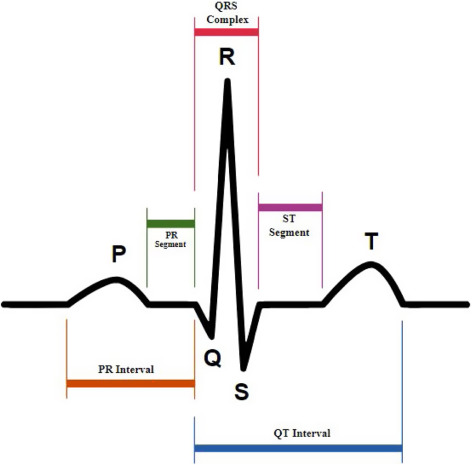
\includegraphics[width=0.7\linewidth,height=0.18\textheight,keepaspectratio]{images/LabelledHeartbeat.jpg}
    \caption[A single PQRST wave]{A single heartbeat with its main waves and intervals. Generated by the author from \cite{Mazomenos_ECG_2012}.}
    \label{fig:ecg-beat}
  \end{minipage}\hfill
  \begin{minipage}[b]{0.52\linewidth}
    \centering
    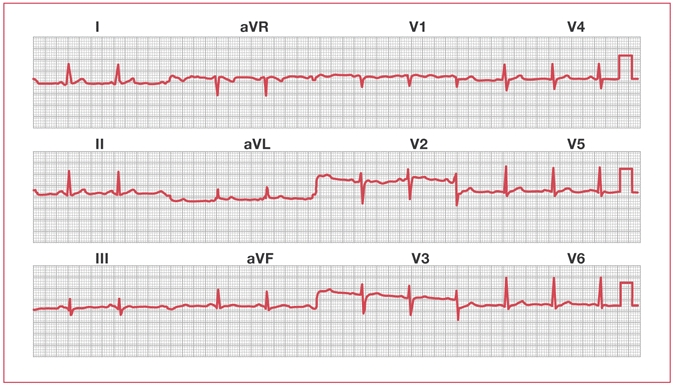
\includegraphics[width=0.7\linewidth,height=0.18\textheight,keepaspectratio]{images/ECGGrid.jpg}
    \caption[An ECG paper trace]{A twelve-lead ECG printed as a $3\times4$ grid of leads \cite{ashley_conquering_2004}.}
    \label{fig:ecg-grid}
  \end{minipage}
\end{figure}

Arrhythmias change the rate or rhythm \cite{nhs_heart_2018}: atrial fibrillation has irregular beats without clear P waves \cite{van_gelder_2024_2024}, and atrial flutter a saw-tooth pattern \cite{cosio_atrial_2017}. Bundle branch blocks widen the QRS complex \cite{scherbak_left_2024}, MI alters the ST segment and T wave, and hypertrophy changes amplitudes \cite{channer_myocardial_2002}. Some classes thus depend on shape and others on timing, which in an image depends on the grid scale. PTB-XL labels 21,800 twelve-lead ECG signals from about 19,000 patients with five diagnostic superclasses (normal, MI, ST/T change, conduction disturbance, hypertrophy) and rhythm statements, allowing several labels per record \cite{wagner_ptbxl_2020}.

\section{ECG Imaging and Digitisation}
\label{sec:ecg-imaging}

Printed or photographed ECGs cannot be used by signal-based software \cite{shivashankara_ecg-image-kit_2024}, and they vary in lighting, artefacts and camera angle \cite{reyna_ecg-image-database_2024}; \textcite{gliner_domain_2023} needed domain adaptation to move a model from scans to phone images, and image resolution limits how accurately timing can be measured. There are two approaches.

\subsection{ECG Digitisation Approach}
\label{sec:digitisation}

Digitisation reconstructs the signal from the image, by locating the grid, separating the leads and tracing each waveform, so that signal-based methods can be applied. It gives measurable intervals, but an error at any step carries into the reconstructed signal. The PhysioNet Challenge 2024 evaluated digitisation by the SNR of the recovered signal \cite{physionet_challenge_2024}.

\subsection{Direct Classification Approach}
\label{sec:direct-classification}

Direct classification avoids reconstruction, but the model must learn timing from pixels, so its results depend on how the images were produced. Two data sources support it: ECG-Image-Kit generates synthesised images with artefacts from real signals \cite{shivashankara_ecg-image-kit_2024}, and the ECG-Image-Database provides about 36,000 images of PTB-XL and Emory Healthcare records that were printed, degraded, and scanned or photographed \cite{reyna_ecg-image-database_2024}; a smaller set of real images with varied degradation is also available \cite{khan_ecg_2021}. This project will classify images directly, training on images rendered from PTB-XL and testing on real images, so that the effect of real imaging conditions can be measured.

\section{Pre-processing and Noise Removal}
\label{sec:preprocessing}

Preprocessing applies the methods of Table~\ref{tab:techniques} to faults from printing and capture, with ECG-specific risks. The grid can confuse a classifier but is the only record of scale, so it must be measured before removal; the trace is only a few pixels wide, so smoothing can erase P waves and QRS peaks; rotation correction cannot fully undo the perspective of a photograph; and a CNN trained on varied images may not need preprocessing at all. Preprocessing will therefore be judged by its effect on classification.

\section{Feature Extraction}
\label{sec:features}

Classical ECG analysis measured hand-designed features, such as interval lengths and wave amplitudes, and passed them to a classifier \cite{de_chazal_automatic_2004}. These have clear clinical meaning, and RR regularity separates regular from irregular rhythms, but they depend on every earlier step succeeding. A CNN instead learns features from the pixels \cite{lecun_deep_2015}, which avoids this dependency but is harder to explain and needs more data. Figure~\ref{fig:feature-extraction} compares the two routes. This project will combine them: learned features suit the shape-based superclasses, and measured timing features (Section~\ref{sec:waveform}) support the rhythm classes.

\begin{figure}[!htbp]
  \centering
  \makebox[\linewidth][c]{%
  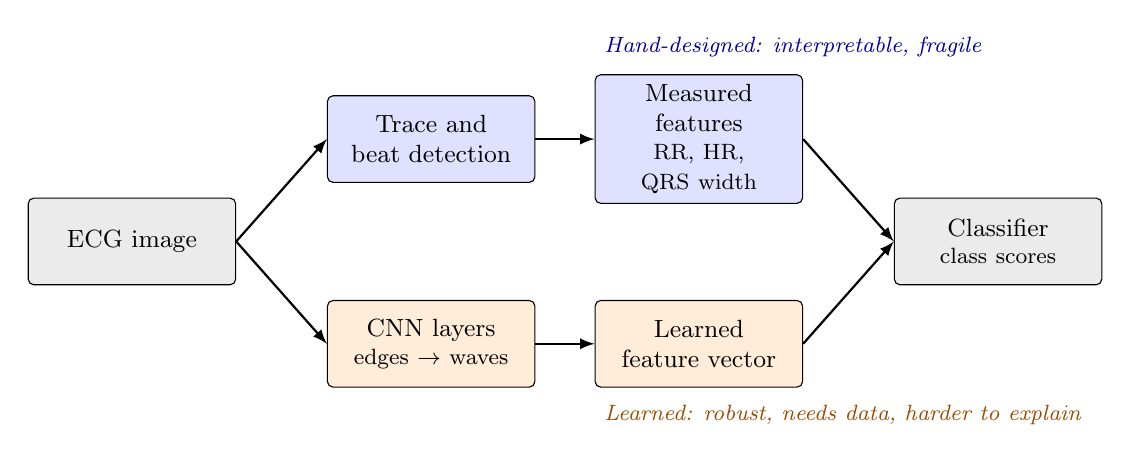
\begin{tikzpicture}[
      font=\small,
      box/.style={draw, rounded corners=2pt, align=center, minimum height=11mm,
                  text width=24mm, fill=#1},
      box/.default=white,
      arr/.style={-latex, thick}
    ]
    \node[box=black!8] (img) at (0,0) {ECG image};
    \node[box=blue!12] (det) at (38mm,13mm) {Trace and beat detection};
    \node[box=blue!12] (meas) at (72mm,13mm) {Measured features\\[-1pt]\footnotesize RR, HR, QRS width};
    \node[box=orange!15] (conv) at (38mm,-13mm) {CNN layers\\[-1pt]\footnotesize edges $\rightarrow$ waves};
    \node[box=orange!15] (learn) at (72mm,-13mm) {Learned feature vector};
    \node[box=black!8] (clf) at (110mm,0) {Classifier\\[-1pt]\footnotesize class scores};

    \draw[arr] (img.east) -- (det.west);
    \draw[arr] (det) -- (meas);
    \draw[arr] (meas.east) -- (clf.west);
    \draw[arr] (img.east) -- (conv.west);
    \draw[arr] (conv) -- (learn);
    \draw[arr] (learn.east) -- (clf.west);

    \node[anchor=south west, font=\footnotesize\itshape, text=blue!60!black]
      at ([yshift=1mm]meas.north west) {Hand-designed: interpretable, fragile};
    \node[anchor=north west, font=\footnotesize\itshape, text=orange!60!black]
      at ([yshift=-1mm]learn.south west) {Learned: robust, needs data, harder to explain};
  \end{tikzpicture}%
  }
  \caption{Hand-designed and learned feature extraction from an ECG image. This project
    will pass timing features from detected beats to the classifier alongside the features the CNN learns.}
  \label{fig:feature-extraction}
\end{figure}

\section{Waveform Detection}
\label{sec:waveform}

In signals, waveform detection usually locates the QRS complex; the Pan--Tompkins algorithm band-pass filters, differentiates and squares the signal, then applies adaptive thresholds \cite{pan_real-time_1985}. In images, the trace must first be found: published pipelines binarise the image, remove the grid and text, locate each lead with a Hough transform, and reduce each column of the trace to one value before converting it to time and voltage \cite{wu_automated_2022}. Detection can be accurate, with correlations of 0.94 \cite{randazzo_development_2022} and about 0.99 on standard layouts \cite{wu_automated_2022} against reference signals, but it is fragile: correlation fell to about 0.96 on printed and rescanned ECGs \cite{wu_automated_2022}, and a missed peak corrupts every timing feature that follows. This project will therefore evaluate detection on real images, not only rendered ones.

\section{ECG Classification Algorithms}
\label{sec:ml-ecg}

Deep learning has largely replaced feature-based ECG classification. On signals, networks reached cardiologist-level rhythm classification (F1 0.837 against 0.780 for cardiologists) \cite{hannun_cardiologist_2019}, outperformed residents on 12-lead abnormalities \cite{ribeiro_automatic_2020}, and convolutional architectures performed best on PTB-XL \cite{strodthoff_deep_2021}. Image-based work is newer and relies on transfer learning from networks such as ResNet pretrained on natural images \cite{he_deep_2016,yosinski_transfer_2014}; the main image-based systems are compared in Section~\ref{sec:existing-systems}, and the key signal and image studies are summarised in Table~\ref{tab:ecg-studies} (Appendix~\ref{app:lit}). Signal results do not transfer directly to images, which carry their scale only through the grid. Labels also limit all studies: PTB-XL's come from at most two cardiologists \cite{wagner_ptbxl_2020}, who can disagree \cite{dhutia_interrater_2017}, and differing datasets and metrics mean headline numbers cannot be ranked directly.

\section{ECG Dataset Evaluation}
\label{sec:ml-eval}

ECG datasets are imbalanced, so accuracy can be high even when rare conditions are missed; sensitivity, specificity and MCC give a truer picture \cite{chicco_advantages_2020}, and data should be split by patient using PTB-XL's suggested folds \cite{wagner_ptbxl_2020}. Overconfident networks can be calibrated by temperature scaling \cite{guo_calibration_2017}: each class score $z_k$ is divided by a temperature $T$ fitted on validation data, $\hat{p}_k = \sigma(z_k/T)$, leaving AUROC unchanged, and calibration is measured by the ECE. Applying this to independent sigmoid outputs is an adaptation, and calibration deteriorates under data shift \cite{ovadia_trust_2019}, so whether it survives the move to real images must be measured. Grad-CAM heatmaps show which regions influenced a prediction \cite{selvaraju_gradcam_2017}, but some saliency maps barely change when a model's weights are randomised \cite{adebayo_sanity_2018}, so heatmaps must be checked against known cases.

\section{Existing Systems and Limitations}
\label{sec:existing-systems}

Most ECGs are analysed by the recording machine's software, but its accuracy is limited, so over-reading by an experienced reader is needed, and it cannot analyse printouts \cite{schlapfer_computer-interpreted_2017}. Table~\ref{tab:existing-systems} compares this with the main deep-learning systems.

\begin{table}[H]
  \centering
  \footnotesize
  \renewcommand{\arraystretch}{1.1}
  \caption{Comparison of existing ECG analysis systems and the planned system.}
  \label{tab:existing-systems}
  \begin{tabular}{@{}p{0.17\linewidth} p{0.17\linewidth} p{0.27\linewidth} p{0.31\linewidth}@{}}
    \toprule
    \textbf{System} & \textbf{Input} & \textbf{Key features} & \textbf{Limitations} \\
    \midrule
    ECG machine software \cite{schlapfer_computer-interpreted_2017} &
      Digital signal at recording &
      Immediate automated report &
      Limited accuracy, needs over-reading; cannot analyse printouts or images \\
    \textcite{sangha_automated_2022} &
      Images generated from signals &
      CNN tested on held-out, external and printed ECGs (AUROC 0.98) &
      Trained on generated images; reports discrimination only, not calibration \\
    \textcite{gliner_domain_2023} &
      Scans; phone-captured frames &
      Domain adaptation from scans to phone images (AUROC 0.91) &
      Phone images made by filming printed pages; six unseen formats tested \\
    \textcite{wang_pipeline_2025} &
      Synthetic and external scanned images &
      Challenge-winning ConvNeXt pipeline (AUROC about 0.97) &
      Evaluated on synthetic PTB-XL images, with possible leakage \\
    \textcite{chen_quantifying_2022} &
      Digital signals &
      Uncertainty estimates for atrial fibrillation; improved calibration &
      Signals only, one condition \\
    \midrule
    This project (planned) &
      Rendered images for training; real images for testing &
      Multi-label CNN with timing features; calibrated confidence; Grad-CAM; views for different users; user study &
      Labels from at most two annotators; real test set limited to the ECG-Image-Database \\
    \bottomrule
  \end{tabular}
\end{table}

Four gaps remain. First, image-based classification has mostly been tested on synthetic or limited real images (Table~\ref{tab:existing-systems}). Second, calibration has been studied for signals \cite{chen_quantifying_2022}, but image-based studies report only discrimination. Third, explanations are seldom assessed: 43\% of explainable-AI studies in cardiology did not evaluate them, and only 11\% involved clinicians \cite{salih_review_2024}. Fourth, presentation depends on the user: clinicians preferred visualisations of what the algorithm analysed \cite{hughes-noehrer_contrasting_2024}, and explanations raised novices' trust more than experts' \cite{cabitza_painting_2023}. Datasets also reflect limited settings: PTB-XL was collected between 1989 and 1996 with devices from one manufacturer \cite{wagner_ptbxl_2020}, so models may not generalise.

\section{Summary}
\label{sec:lit-summary}

Reading an ECG from an image combines an image problem, recovering a measurable trace from a degraded picture, with a clinical problem, deciding what the trace shows. Signal-based deep learning is mature, but image-based work has relied on synthetic data and paid little attention to whether its confidence can be trusted or its explanations understood. This project will address the four gaps in turn: a preprocessing and detection pipeline tested on real images, a calibrated multi-label classifier evaluated with imbalance-aware metrics, and an application that presents explained results to different users. Chapter~\ref{ch:method} sets out how.